\chapter[Referencial Teórico]{Referencial Teórico}

"Este capítulo tem como objetivo apresentar o referencial teórico que embasa a pesquisa deste trabalho, incluindo conceitos que serão utilizados para a construção da proposta de trabalho a ser realizado."

\section{Arquitetura de Software}
Existe na literatura, e também é de senso comum da área de tecnologia da informação, a assertiva de que o produto de software é construído com base em uma oportunidade de negócio ou uma necessidade de usuário(s) identificada. Estes produtos de software possuem uma arquitetura associada à sua construção, que é uma composição de estruturas de um ou mais sistemas que exibem não apenas as características visíveis de elementos que o compõem, mas também o relacionamento entre estes elementos \cite{bass_software_archi_practice_2003}.

A arquitetura de software pode ser vista como uma ponte que conecta as necessidades de usuário ou as oportunidades de negócio identificadas ao produto de software construído. Tal arquitetura representa uma abstração do sistema de software a ser desenvolvido e exibe os detalhes que o arquiteto de software julga como necessários. Desta forma, quaisquer produtos de software possuem uma aruiteura definida, independentemente de terem passado pelos processos de desenho, documentação e análise ou não \cite{bass_software_archi_practice_2003}.

Bass, Clements e Kasman\cite{bass_software_archi_practice_2003} definem arquitetura de software como "a estrutura ou conjunto de estruturas de um sistema que comprime os elementos de um software, as propriedades externamente visíveis de tais elementos e os relacionamentos entre eles". Desta definição é possível inferir que sistemas podem ser construídos utilizando-se mais de uma estrutura; que os elementos que compõem o sistema, mas que não interagem diretamente, são omitidos na arquitetura; que também faz parte da arquitetura o comportamento e interação dos elementos; e que, como mencionado anteriormente, todo sistema ou produto de software possui uma arquitetura \cite{bass_software_archi_practice_2003}.

Ainda de acordo com as ideias expostas por \cite{bass_software_archi_practice_2003}, autores importantes na área de arquitetura de software, a definição formal da arquitetura de um software tem sua importância quando o assunto é a comunicação entre envolvidos e decisões importantes: colabora na comunicação entre as partes envolvidas e na tomada de decisões ainda no início do projeto de software, permitindo que outros sistemas possam utilizar abstrações semelhantes.

\subsection{Estilos Arquiteturais}
Segundo Pressman \cite{pressman2006engenharia}, estilos arquiteturais são utilizados para guiar o desenvolvimento de software e podem ser combinados a fim de obter um estilo próprio para cada produto de acordo com os requisitos e restrições identificadas. A seguir, estão descritos alguns dos estilos arquiteturais existentes e descritos na literatura.

\subsubsection{Arquitetura Baseada em Camadas}
A arquitetura baseada em camadas é caracterizada pela divisão de elementos em grupos que possuem responsabilidades semelhantes. Estes grupos compõem camadas da aplicação e estas conversam entre si através de um protocolo estabelecido pelo estilo arquitetural, onde, geralmente, uma camada interage apenas com camadas mais próximas \cite{pressman2006engenharia}. A figura a seguir é uma ilustração deste estilo.

\begin{figure}[htb]
\centering
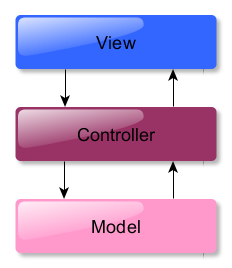
\includegraphics[scale=0.5]{figuras/modelo_mvc.PNG}
\caption{Padrão MVC - Arquitetura baseada em camadas.}
\label{modelo_mvc}
\end{figure}

A figura acima exibe o padrão arquitetural MVC - \textit{Model View Controller} -, que é uma implementação do estilo arquitetural baseado em camadas. No MVC, a camada de modelo (\textit{Model}) interage apenas com a camada de controle (\textit{Controller}). Esta, por sua vez, é responsável por promover a interação entre as camadas \textit{View} e \textit{Model}.

\subsubsection{Arquitetura Orientada a Serviços}

Este é um estilo que promove a interoperabilidade de um dado sistema, permitindo troca de dados e interação entre diversas aplicações independentemente das plataformas em que são executadas ou tecnologias utilizadas para a sua construção \cite{oqueesoa_2010}

Na arquitetura orientada a serviços, as funcionalidades ou módulos de um sistema são definidos como um serviço. Os serviços disponibilizados são expostos através do estabelecimento de contratos e interfaces de acesso e requisitados por meio do envio e recebimento de mensagens pelas aplicações \cite{oqueesoa_2010}.

\subsubsection{Arquitetura Cliente-Servidor}
O estilo arquitetural cliente-servidor é utilizado como um modelo para a implementação de sistemas distribuídos. Neste estilo, os clientes são responsáveis por realizar requisições a um conjunto de servidores que disponibilizam serviços. Geralmente, os clientes se comunicam de maneira direta com os servidores e possuem conhecimento apenas dos servidores disponíveis, desconhecendo os outros clientes existentes. Um exemplo de implementação deste estilo é a rede de uma organização onde os usuários (clientes) têm conhecimento acerca de impressoras (servidores) disponíveis. Ao acionar o serviço de impressão, o cliente estebelece uma comunicação direta com a impressora \cite{sommerville2008engenharia}.

\subsubsection{Arquitetura Baseada em Eventos}
A arquitetura baseada em eventos é um estilo arquitetural onde ocorrências importantes no sistema são identificados pelo software ou hardware que o compõe. É composta por elementos que criam um evento, que apenas sabem que um evento ocorreu e o anuncia aos demais elementos do sistema, e por aqueles que consomem os eventos anunciados. Os elementos consumidores necessitam dos eventos para realizar o processamento de uma determinada operação ou mudança de estado \cite{rouse}.

\section{SOA - Arquitetura Orientada a Serviços}

Sendo tratado como um conceito evolucionário, a orientação a serviços é uma abordagem que foi criada para a construção de sistemas de software distribuídos, a fim de promover a integração com baixo acoplamento entre aplicações e facilitar a manutenção corretiva, adaptativa ou evolutiva das mesmas \cite{linthicum_soainrealworld_2007}. Em outras palavras, a arquitetura orientada a serviços, também conhecida como SOA - do acrônimo em inglês \textit{Service-Oriented Architecture} - é "um paradigma para a construção e manutenção de processos de negócio que conecta sistemas distribuídos" \cite{josuttis_soa_2007}.

Este modelo arquitetural é utilizado para o desenho, construção, implantação e gerenciamento de sistemas de software, onde as funcionalidades deste sistema são providos por serviços que possuem interfaces de acesso bem definidas \cite{lewis_getting_2010}. Desta forma, podemos afirmar que SOA não é um tipo de tecnologia, ferramenta ou processo a serem utilizados para a construção de software, mas uma abordagem utilizada para a definição e construção da arquitetura de determinadas aplicações \cite{oliveira_interoperabilidade}.

De acordo com Josuttis \cite{josuttis_soa_2007}, SOA é um recurso a ser utilizado para construir uma arquitetura de software concreta e tem como objetivo melhorar a flexibilidade de um sistema de software, baseando-se em três conceitos técnicos principais: serviços, interoperabilidade promovida por um barramento de serviços e baixo acoplamento. SOA é uma abordagem adequada para a implementação de sistemas distribuídos em que sistemas heterogêneos são aceitos, ou seja, aplicações desenvolvidas em plataformas diferentes e em linguagens de programação distintas são capazes de interagirem formando um sistema único \cite{josuttis_soa_2007}.

A indústria de software frequentemente implementa o modelo SOA utilizando Web Services que são, de acordo com a W3C \cite{haas_web_2004}, sistemas de software construídos para dar suporte à interação ponto-a-ponto de maneira interoperável através da rede. Contudo, a orientação a serviços é algo independente de tecnologias e padrões, justificando sua implementação quando sistemas legados devem ser incorporados à arquitetura de um sistema de software \cite{linthicum_soainrealworld_2007}. A implementação deste modelo pode combinar diversas tecnologias, APIs, diferentes composições de infra-estrutura, constituindo sempre uma arquitetura única \cite{erl_orientacaoaservico_2009}.

Como qualquer modelo, SOA apresenta benefícios para a construção de software e características que podem ser ditas como desvantajosas quando este modelo é utilizado. A integração com  outros serviços, aplicativos e sistemas legados, além de prover um investimento de retorno elevado, a reutilização, flexibilidade, intereoperabilidade e governança de um serviço caracterizam algumas das vantagens relacionado ao uso este modelo \cite{oqueesoa_2010} \cite{vantagens_desvantagens_soa}. As desvantagens identificadas estão relacionados a segurança de acesso, complexidade devido à quantidade de serviços (quanto mais robusta, ou seja, quanto mais serviços, mais complexa será a arquitetura construída), performance do servidor que afeta a disponibilidade do sistema de software e a testabilidade deste  \cite{oqueesoa_2010} \cite{vantagens_desvantagens_soa}.

\subsection{Conceitos Principais}
\subsubsection{Serviços}

Serviço pode ser definido como uma aplicação de software que interage com outras aplicações por meio da troca de mensagens \cite{linthicum_soainrealworld_2007}. Além disso, um serviço é uma coleção de capacidades \cite{erl_orientacaoaservico_2009}, "é um valor entregue para outro (serviço) através de uma interface bem definida e disponível e resulta em um trabalho provido de um para outro" \cite{adaptive_ltd_service_2009}.

Um serviço é uma aplicação independente e deve ser composto por duas partes principais: a interface, que permite a comunicação com os usuários do serviços e define a estrutura das mensagens a ser utilizada para a comunicação entre um serviço e seu usuário; e a implementação, que consiste do núcleo do serviço, desconhecido pelo usuário, mas a parte responsável pela execução do serviço \cite{linthicum_soainrealworld_2007} . As principais características de um serviço, de acordo com Jossutis \cite{josuttis_soa_2007} e Erl   \cite{erl_orientacaoaservico_2009}, são:

\begin{itemize}
\item Um serviço deve ser \textbf{autônomo},  capaz de controlar seu ambiente e recursos disponibilizados. Isto implica na não interferência de fatores externos à aplicação que implementa o serviço, dependendo apenas de parâmetros fornecidos pelos usuários de um dado serviço.

\item Um serviço deve estar sempre \textbf{visível e disponível} para que possa ser descoberto e utilizado por seus usuários.

\item Um serviço deve possuir uma \textbf{alta abstração}, de modo que os detalhes de implementação sejam ocutados e apenas a interface seja acessível.

\item Um serviço \textbf{não deve guardar} informações sobre o \textbf{estado} de requisições anteriores. Informações acerca do estado de um serviço deve ser mantida apenas quando necessário.

\item Um serviço deve ser construído de modo que possa ser \textbf{reutilizado} por outras aplicações.

\item Um serviço pode ser construído a partir da \textbf{composição de outros serviços}.

\item Um serviço deve ser \textbf{idempotente}, isto é, ao ser utilizado um serviço deve retornar sempre o mesmo resultado quando os recursos disponibilizados para a sua execução forem os mesmos.

\item Um serviço deve possuir um \textbf{contrato de serviço padronizado}, que expressa o objetivo e a capacidade que o serviço implementa.
\end{itemize}

Algumas destas características podem ser inferidas a partir da imagem a seguir.

\begin{figure}[htb]
\centering
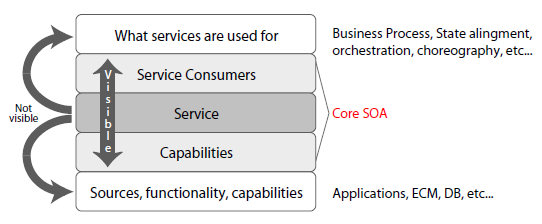
\includegraphics[scale=0.8]{figuras/servico_na_arquitetura.png}
\caption{Serviço em uma arquitetura baseada no modelo SOA. Fonte: \cite{nickull_service_2007}.}
\label{servico_na_arquitetura}
\end{figure}

A figura acima expressa o serviço como o núcleo de uma arquiteura baseada no modelo SOA. As capacidades de um serviço, o próprio serviço e os consumidores deste serviço formam o núcleo deste modelo, sendo visíveis e transparentes em uma arquitetura de software. Como um serviço deve ocutar seus detalhes de implementação e geralmente não possui conhecimento do sistema de software em que está inserido \cite{nickull_service_2007}.

\subsubsection{Baixo Acoplamento}
O baixo acoplamento permite que a dependência entre sistemas de software seja reduzido. Isto pode ser implementado de duas maneiras distintas: uma utiliza a comunicação assíncrona entre aplicações e a outra faz uso de compensação para manter a consistência do estado dos sistemas de software que utilizam e fornecem serviços \cite{josuttis_soa_2007}.

A maior desvantagem de um sistema onde os níveis de acoplamento são baixíssimos é a complexidade, elevando a dificuldade para desenvolver, manter e \textit{debugar} a arquitetura criada \cite{josuttis_soa_2007}.

\subsubsection{Interoperabilidade}
Josuitts \cite{josuttis_soa_2007} define a interoperabilidade como "a habilidade de sistemas diferentes se comunicarem", independentemente das tecnologias e linguagens de programação utilizadas na construção de tais sistemas de software. Existem padrões relacionados à interoperabilidade entre sistemas de software, que não necessariamente garantem, mas colaboram na implementação desta característica. 

Os padrões de interoperabilidade existentes, também conhecidos como WS-I, visam segundo Oliveira e Navarro \cite{oliveira_interoperabilidade}, a integração de especificações, promoção de implementações consistentes e que sigam guias e boas práticas, o fornecimento de ferramentas e aplicações como referências e o encorajamento da adoção de tais padrões. Os principais padrões WS-I são:

\begin{itemize}
\item \textit{WS-Addressing}: visa uma solução que garanta que a origem e o destino das mensagens trocadas pelas aplicações sejam endereçadas de forma independente do meio de transporte \cite{oliveira_interoperabilidade}.
\item \textit{WS-Policy}: permite a adição de politicas a serem cumpridas por clientes e provedores do serviço visando a efetividade da interação entre estes \cite{oliveira_interoperabilidade}.
\item \textit{WS-Transaction}: padrão que define como se dará a interoperabilidade entre diferentes Web Services para "compor a qualidade de serviços transacionais entre aplicações" \cite{oliveira_interoperabilidade}.
\item \textit{WS-Security}: fornece segurança a nível de mensagem, garantindo a confidencialidade e integridade das mensagens, uma vez que estas passam por diversos sistemas intermediários entre a sua origem e o seu destino. Os mecanismos de segurança devem ser utilizados apenas quando realmente necessários já que o consumo de processamento pode aumentar, afetando o tempo de resposta de um serviço \cite{oliveira_interoperabilidade}.
\end{itemize}

Quando os serviços seguem padrões independentes da tecnologia, permitindo que a utilização seja transparente e fácil para diversos clientes que utilizam diferentes tecnologias diz-se que interoperabilidade existe neste contexto, fornecendo uma abstração que colabora para o baixo acoplamento entre as aplicações \cite{oliveira_interoperabilidade}.

\subsection{Modelos de integração}
A integração entre os subsistemas de software que compõem a arquitetura distribuída de um sistema construído com base no modelo arquitetural SOA pode ser estabelecida usando-se diferentes estatégias. A estratégia utilizada para promover tal integração é um aspecto que deve ser cuidadosamente analisado, pois o impacto de tal decisão é importante e irá perpertuar-se durante a existência do produto final de software construído. Desta forma, de acordo com Bianco et. al. \cite{Bianco2007} existem duas principais abordagens para a integração entre os sistemas que compõem a implementação deste modelo:

\begin{figure}[htb]
\centering
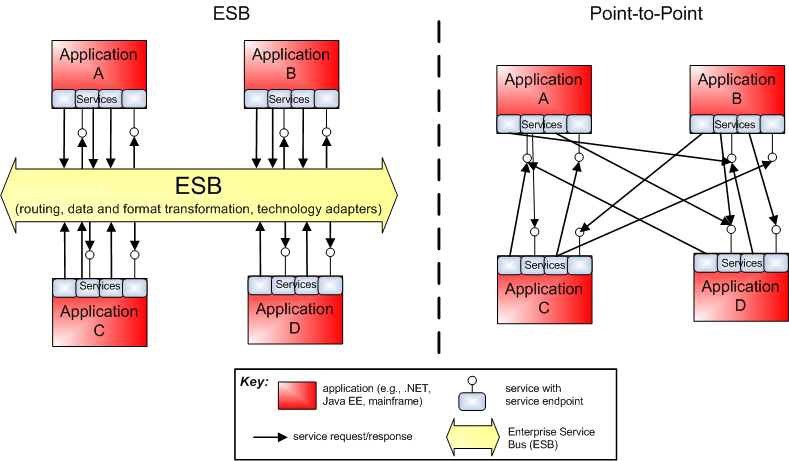
\includegraphics[scale=0.7]{figuras/modelos_integracao_soa.png}
\caption{Ilustração dos modelos de integração em SOA. Fonte: \cite{Bianco2007}.}
\label{modelos_integracao_soa}
\end{figure}

\begin{itemize}
\item \textbf{Direto (Ponto-a-Ponto)}: a interface de comunicação é única entre usuários e provedores de serviço; as questões relacionadas a conectividade entre os sistemas devem ser de reponsabilidade compartilhada entre tais aplicações.
\item \textbf{\textit{Hub-and-Spoke}}: a comunicação entre usuários e provedores de serviço é mediada por um terceiro software chamado ESB (\textit{Enteprise Service Bus}) ou EAI (\textit{Enterprise Application Integration}); nesta abordagem, as aplicações estebelecem uma comunicação com o ESB (ou EAI), responsável por gerenciar as mensagens enviadas pelas aplicações.
\end{itemize}

\subsection{ESB - Enterprise Service Bus}

O ESB, ou \textit{Enterprise Service Bus}, consiste em um barramento de serviços cuja principal responsabilidade é promover a interoperabilidade do sistema de software que implementa o modelo SOA \cite{josuttis_soa_2007}. A criação do ESB foi uma solução encontrada para reduzir a quantidade de interfaces e canais de comunicação a serem mantidos quando o sistema de software construído constitui uma aplicação distribuída: a interface tanto dos serviços quanto das aplicações usuárias estabelecem uma comunicação apenas com o barramento, não necessitando mais se adaptarem a cada interface definida pelos serviços existentes e que fazem parte do sistema \cite{josuttis_soa_2007}.

A conexão entre provedores e usuários de serviços é realizada através deste \textit{middleware} e de forma padronizada, sendo que a utilização de uma ferramenta que provê os recursos propostos para que tal consista de um ESB (tratados logo adiante) não é uma obrigatoriedade para que uma arquitetura construída implemente o modelo SOA \cite{lewis_getting_2010}.

Como citado anteriormente, o uso de um ESB possui como principal objetivo a promoção de interoperabilidade de um sistema de software. Segundo Josuttis \cite{josuttis_soa_2007}, para atingir estes objetivos, um ESB deve ser capaz de:

\begin{itemize}
\item Prover conectividade entre provedor e consumidor do serviço.
\item Realizar transformação de dados
\item Fazer o roteamento das mensagens (tanto requisições quanto respostas)
\item Lidar com confiança e segurança de dados
\item Gerenciar os serviços conhecidos pelo ESB.
\item Monitorar e manter registros das transações
\end{itemize}

Sendo um conceito relacionado ao modelo SOA, o ESB também possui padrões que devem ser seguidos quando deseja-se implementar uma ferramenta caracterizada pelos requisitos descritos. A imagem a seguir ilustra os padrões indicados.

\begin{figure}[htb]
\centering
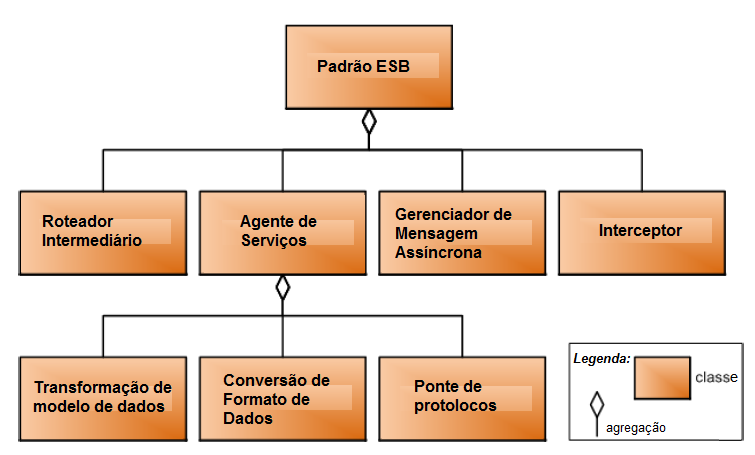
\includegraphics[scale=0.5]{figuras/padrao_ESB.png}
\caption{Ilustração de padrões ESB. Fonte: \cite{bianco_architecting_2011}.}
\label{padrao_ESB}
\end{figure}

A imagem acima exibe os principais componentes de um ESB: roteador intermediário, intermediador ou agente de serviços (\textit{service broker}), um agente responsável por gerenciar mensagens assíncronas e um interceptor. Como exposto por Bianco et. al. \cite{bianco_architecting_2011}, as principais características de cada um destes componentes são:

\begin{itemize}
\item Roteador intermediário: componente capaz de receber mensagens de requisição e resposta e determinar o serviço ou aplicação que deverá receber tal mensagem.
\item Service Broker (ou agente de serviços): realiza o tratamento adequado das mensagens dentro do ESB. Este componente é formado por estruturas responsáveis pela transformação do modelo de dados, conversão dos formatos de mensagens recebidas pelo ESB para o formato suportado pelo serviço ou aplicação, além da conversão de protocolos quando aqueles utilizados pelo provedor e usuário do serviço são distintos.
\item Gerenciador de mensagem assíncrona: nem sempre os canais de comunicação realizam a troca de mensagens de forma síncrona. O papel deste componente é gerenciar as mensagens de requisições e respostas de transações assíncronas.
\item Interceptor: é o elemento responsável por receber as mensagens que chegam ao ESB.
\end{itemize}

\subsubsection{WSO2 ESB}
Uma das ferramentas que implementam os padrões estabelecidos para o ESB é a WSO2 ESB. Esta é uma ferramenta \textit{open source} e foi construída a partir da licença Apache 2.0. Entre as principais características desta ferramenta estão o suporte para transformação/conversão, roteamento e validação de mensagens, troca de protocolos de comunicação, exposição de sistemas legados, políticas de autenticação e autorização para acesso aos serviços, além de permitir o monitoramento das transações realizadas e o armazenamento de mensagens \cite{siriwardena_enterprise_2013}.

\subsubsection{JBoss ESB}
O JBoss ESB é uma implementação dos padrões e abordagens relacionados ao conceito de ESB. Esta é uma ferramenta, também do tipo \textit{open source}, que consiste em um barramento de serviços onde as mensagens trocadas através deste podem passar por processos de conversão de formatos, dados e protocolos de comunicação, além de realizar o roteamento das mensagens com o auxílio de componentes, tais como conectores e adaptadores, que colaboram para a rápida criação de canais de comunicação entre as aplicações conectadas ao barramento de maneira facilitada \cite{silva_jbossesb_2008}.

\subsubsection{ErlangMS}
ErlangMS é um ESB open source desenvolvido na linguagem Erlang durante a realização de uma tese de mestrado na Universidade de Brasília. A proposta deste barramento é "fornecer uma camada de serviço em uma implementação do modelo SOA" para a integração dos sistemas implanatados na instituição. Esta implementação do ESB possui, além dos padrões definidos para este conceito, características relacionadas à estrutura de eventos (onde eventos ocorridos em dada aplicação são anunciados às outras através do barramento) e recursos de tolerância a falhas \cite{agilar_uma_2015}.

\section{Protocolos de Comunicação}
Um protocolo de comunicação é definido na literatura como um conjunto de regras que determinam o formato e o significado de pacotes de mensagens (ou apenas mensagens) que são transferidos entre aplicações ou sistemas \cite{Stallings_2006}. Desta forma, é possível afirmar que sistemas de software utilizam protocolos para estabelecer uma comunicação entre as entidades do sistema e implementar as definições de serviço que são fornecidas por cada entidade \cite{Stallings_2006}.

Protocolos de comunicação são formados por três elementos principais: sintaxe, semântica e temporizador. A sintaxe consiste no elemento responsável por definir o formato das mensagens ou pacotes que serão enviados e recebidos por um sistema ou serviço. O controle da informação e o tratamento de erros na troca de dados entre elementos de um sistema que utiliza um protocolo de comunicação são atividades realizadas pelo elemento semântico de um protocolo. O temporizador é responsável por gerenciar a velocidade e o sequenciamento de dados que são enviados e recebidos \cite{Stallings_2006}.

A troca de mensagens entre aplicações podem ser realizadas de diferentes formas e seguir padrões jpa conhecidos e estabelecidos, e que influenciam na definição do protocolo de comunicação. Os padrões expostos por Josuttis \cite{josuttis_soa_2007} são quatro: \textit{request/response}, \textit{one-way}, \textit{request/callback} e \textit{publish/subcribe}.

O padrão de comunicação \textit{request/response} permite a troca síncrona de mensagens, onde as respostas geradas pelo processamento de requisição são imediatamente encaminhadas à aplicação que inicializou a comunicação. Esta, por sua vez, mantém-se em estado de espera pela resposta \cite{josuttis_soa_2007}. O padrão \textit{one-way} é mais utilizado para o envio de notificações, não sendo necessário o envio de uma mensagem de resposta (como sugerido pelo próprio nome do padrão) \cite{josuttis_soa_2007}. Estes padrões estão ilustrados na imagem abaixo.

\begin{figure}[htb]
\centering
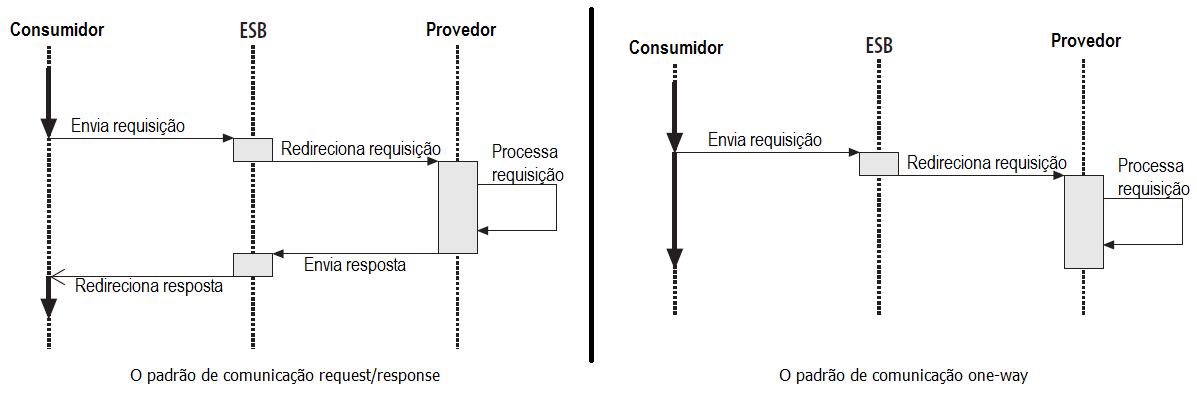
\includegraphics[scale=0.5]{figuras/padroes_comunicacao.png}
\caption{Ilustração de padrões de comunicação. Fonte: \cite{josuttis_soa_2007}.}
\label{padroes_comunicacao}
\end{figure}

O padrão conhecido como \textit{request/callback} é utilizado quando a troca de dados entre duas aplicações ocorrem de forma assíncrona, permitindo que o processo que realizou a requisição não permaneça bloqueado até que a resposta seja recebida. Este tipo de troca de mensagens colabora no baixo acoplamento entre aplicações, uma vez que a aplicação que realiza a requisição não permanece bloqueada quando mensagens são enviadas a provedores de serviço indisponíveis \cite{josuttis_soa_2007}. No entanto, a aplicação usuária de serviços deve tratar o recebimento de mensagens de maneira adequada devido ao fato de que nem sempre a ordem de recebimento das respostas é corresponde àquela de envio de requisições \cite{josuttis_soa_2007}.

Também conhecido como \textit{observer}, o padrão \textit{publish/subcribe} permite que vários observadores realizem uma espécie de "inscrição" em um sistema e sejam notificados quando um dado evento ocorre  \cite{josuttis_soa_2007}.

\subsection{SOAP}
Uma das abordagens de comunicação utilizadas em sistemas que implementam a arquitetura SOA é realizado com o uso de SOAP - Simple Objects Access Protocol. Este é um protocolo centrado em operações diversas a serem executadas pelo provedor de serviços. De acordo com a definição da W3C \cite{box_simple_2000}, este "é um protocolo para troca de informações em sistemas distribuídos, baseado em XML e consiste de três partes principais: definição de um \textit{framework} das mensagens trocadas e o método de processamento destas, um conjunto de de regras para codificação das mensagens e dados nestas contidos e um padrão para a realização de procedimentos e envio de respostas".

As definições de interface de um serviço que utiliza o modelo SOAP para troca de mensagens é feita por meio do uso da linguagem WSDL (\textit{Web Services Definition Language}), onde são declarados dois atributos que definem como será, de fato, a comunicação: estilo e uso. O estilo define a estrutura da mensagem e podem ser "RPC" (\textit{Remote Procedure Call}), onde nomes e tiposdos argumentos são bem definidos, ou "\textit{document}", onde um documento de conteúdo qualquer é encapsulado em um arquivo XML. O uso estebelece se a mensagem deve ser codificada ("\textit{encoded}") ou enviada de maneira literal ("\textit{literal}") \cite{Bianco2007}.

Sendo apenas um protocolo de comunicação, que define o formato e organização dos dados das mensagens, esté é dependente de um protocolo de transporte para que as mensagens trocadas com o uso de SOAP sejam conduzidas da sua origem até o seu destino. Mensagens no padrão SOAP são comumente enviadas utilizando-se o protocolo HTTP de transporte, mas também é suportada por outros protocolos, como o SMTP (\textit{Simple Mail Transfer Protocol}) e JMS (\textit{Java Message Service}) \cite{mueller_understanding_2013}.

\subsection{REST}
Como opção de uma abordagem mais simples de comunicação entre entidades que compõem um sistema de software baseado em serviços e de fácil entendimento e acessibilidade, existe o REST (Representational State Transfer). O uso desta abordagem é baseado no conceito de acesso à recursos ou informações fornecidas por serviços através do uso de APIs ou \textit{Web Services} \cite{Bianco2007}. Este modelo faz uso de apenas dois métodos de transporte: HTTP e HTTPS \cite{rozlog_restesoap_2013}.

Sendo baseado no acesso à recursos e informações e utilizando HTTP (e HTTPS) como protocolo de transporte, o REST suporta apenas chamadas de operações básicas como GET, PUT, POST, DELETE e estas requisições devem ser realizadas via URL \cite{rozlog_restesoap_2013}.

Embora o protocolo de transporte seja limitado a apenas um tipo, variando apenas com relação a critérios de segurança de rede, o REST suporta vários formatos de mensagens, geralmente resultados de requisições realizadas com o uso de uma URL específica, onde os parâmentos necessários para o processamento da requisição são também indicados. Os formatos de mensagem suportados são CSV, JSON e RSS \cite{mueller_understanding_2013}, além de permitir o uso de objetos XMLHttpRequest (API em linguagem de \textit{script} para navegadores web) \cite{rozlog_restesoap_2013}.

Esta abordagem é indicada para operações que não necessitam que dados sobre requisições anteriores sejam guardadas, também conhecidas como operações \textit{stateless} \cite{rozlog_restesoap_2013}. Em situações onde os recursos de infraestrutura são limitados e o armazenamento de dados em cache é necessário, recomenda-se o uso do REST \cite{rozlog_restesoap_2013}.

\section{Implementações do modelo SOA existentes}

\subsection{PSOA - Um \textit{framework} de práticas e padrões SOA para projetos DDS}

Esta tese de mestrado, escrita por Pereira \cite{pereira_psoa_2011}, tem como objetivo a construção de um \textit{framework} conceitual que tem como base práticas de desenvolvimento utilizando o modelo SOA para o desenvolvimento de software (referenciado pelo acrônimo DDS).

A fim de alcançar tal objetivo, Pereira \cite{pereira_psoa_2011} realizou um levantamento sobre as práticas e padrões utilizados pela Engenharia de Software, tais como processos e modelos de desenvolvimento de software, definições, visões e padrões de arquitetura de software. Também foi realizado um levantamento de estratégias adotadas por profissionais inseridos no mercado de desenvolvimento de software por meio de entrevistas. Este levantamento de dados ocorreu com profissionais envolvidos no desenvolvimento de software de maneira geral e também com aqueles envolvidos no desenvolvimento de software baseados no modelo SOA.

O \textit{framework} foi construído com base nas boas práticas levantadas através da pesquisa bibliográfica e das entrevistas realizadas. Estão envolvidos no \textit{framework} conceitos que colaboram para que o acesso aos serviços seja de maneira segura, a interação entre usuários e provedores de serviços possa ser também assíncrona, protocolos de comunicação sejam traduzidos quando necessário, aplicações clientes possam ser notificados quando determinados eventos ocorrem (padrão \textit{publisher/subscriber}), aplicações que fornecem serviços exponham múltiplos contratos de serviço (isto permite que um serviço seja utilizado por diversos consumidores), além de permitir o registro de erros e a adaptação de serviços por meio do uso de \textit{Service Façade}.



\section{Engenharia de Software}

\subsection{Conceitos de ESW adotados}
- RUP
- Scrum